\documentclass[tikz]{standalone}
\usepackage{amsmath}
\usepackage{color,pxfonts,fix-cm}
\usepackage{latexsym}
\usepackage{helvet}
\usepackage{lmodern}
\usepackage{fontspec}
\usepackage[T1]{fontenc}
\usepackage[utf8x]{inputenc}
\usepackage{tgpagella}
\usepackage{pict2e}
\usepackage{wasysym}
\usepackage[english]{babel}
\usepackage{tikz}
\usepackage{circuitikz}
\pagestyle{empty}
\usepackage[margin=1in]{geometry}
\usepackage{pgf}
\usepackage{pgfplots}

% Documento
\begin{document}
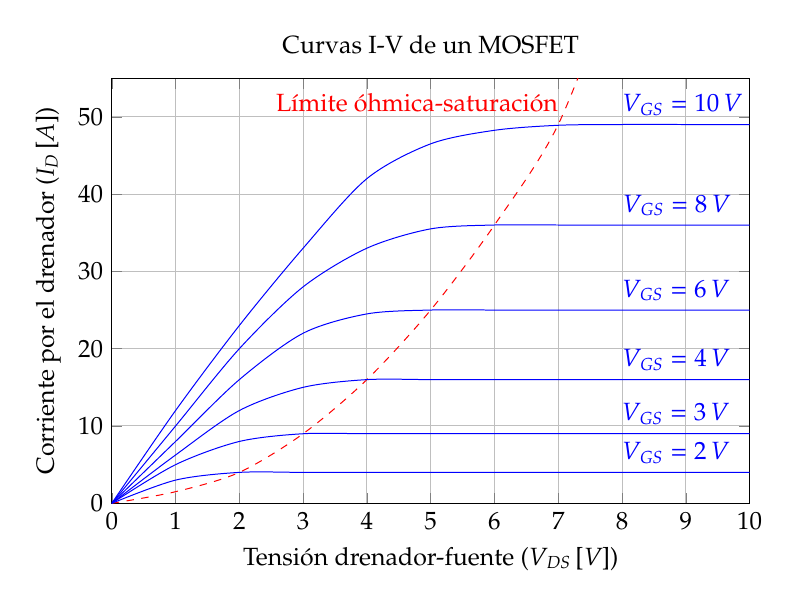
\begin{tikzpicture}[scale=0.9]
    \begin{axis}[%
        title={Curvas I-V de un MOSFET},
        width=9cm,
        height=6cm,
        grid=major,
        scale only axis,
        xmin=0,
        xmax=10,
        ymin=0,
        ymax=55,
        xlabel={Tensión drenador-fuente ($V_\textit{DS}\,[\textit{V}]$)},
        ylabel={Corriente por el drenador ($I_\textit{D}\,[\textit{A}]$)},
    ]
    \addplot [color=red, smooth, dashed, forget plot]
      table[row sep=crcr]{%
    0	0\\
    1   1.5\\
    2   4\\
    3   9\\
    4   16\\
    5   25\\
    6   36\\
    7   49\\
    8   70\\
    }node[pos=0.7425, left]{Límite óhmica-saturación};
    \addplot [color=blue, smooth, forget plot]
      table[row sep=crcr]{%
    0	0\\
    1   12\\
    2   23\\
    3   33\\
    4   42\\
    5   46.5\\
    6   48.25\\
    7   48.9\\
    8   49\\
    9   49\\
    10  49\\
    }node[pos=0.98, above]{$V_\textit{GS}=10\,\textit{V}$};
    \addplot [color=blue, smooth, forget plot]
      table[row sep=crcr]{%
    0	0\\
    1   10\\
    2   20\\
    3   28\\
    4   33\\
    5   35.5\\
    6   36\\
    7   36\\
    8   36\\
    9   36\\
    10  36\\
    }node[pos=0.972, above]{$V_\textit{GS}=8\,\textit{V}$};
    \addplot [color=blue, smooth, forget plot]
      table[row sep=crcr]{%
    0	0\\
    1   8\\
    2   16\\
    3   22\\
    4   24.5\\
    5   25\\
    6   25\\
    7   25\\
    8   25\\
    9   25\\
    10  25\\
    }node[pos=0.9625, above]{$V_\textit{GS}=6\,\textit{V}$};
    \addplot [color=blue, smooth, forget plot]
      table[row sep=crcr]{%
    0	0\\
    1   6.25\\
    2   12\\
    3   15\\
    4   16\\
    5   16\\
    6   16\\
    7   16\\
    8   16\\
    9   16\\
    10  16\\
    }node[pos=0.949, above]{$V_\textit{GS}=4\,\textit{V}$};
    \addplot [color=blue, smooth, forget plot]
      table[row sep=crcr]{%
    0	0\\
    1   5\\
    2   8\\
    3   9\\
    4   9\\
    5   9\\
    6   9\\
    7   9\\
    8   9\\
    9   9\\
    10  9\\
    }node[pos=0.93, above]{$V_\textit{GS}=3\,\textit{V}$};
    \addplot [color=blue, smooth, forget plot]
      table[row sep=crcr]{%
    0	0\\
    1   3\\
    2   4\\
    3   4\\
    4   4\\
    5   4\\
    6   4\\
    7   4\\
    8   4\\
    9   4\\
    10  4\\
    }node[pos=0.9075, above]{$V_\textit{GS}=2\,\textit{V}$};
    \end{axis}
\end{tikzpicture}%
\end{document}